\documentclass[final, 12pt, aspectratio=169, xcolor={dvipsnames}]{beamer}
\usepackage{lmodern}
\usepackage[utf8]{inputenc}
\usepackage[T1]{fontenc}
\usepackage{graphicx} 
\usepackage{textpos} % package for the positioning
%\usepackage{xcolor}
\usepackage{tcolorbox}
\usepackage{tabularx}
\usepackage{hanging}
\usepackage{animate}
\usepackage{caption}

\title[PEARL]{Hoe veel mensen zijn door het coronavirus overleden? Een tijdsreeksanalyse met inschatting van onzekerheid}
\subtitle[PEARL]{}
\author[T. Husby]{Trond Husby, Hans Visser, Lenny Stoeldraijer (CBS) }
\institute[PBL]{
  Netherlands Environmental Assesment Agency (PBL) \\[5ex]
  \texttt{trond.husby@pbl.nl}
}
\date[\today]{Amsterdam 9 Juni, 2020}

% set path to figures
\newcommand*{\figs}{../figs}%

% position the logo
\addtobeamertemplate{background}{}{%
  %\begin{textblock*}{100mm}(0.95\textwidth, 7cm)
  %\begin{flushright}
    
\includegraphics[width=\paperwidth, height=\paperheight]{\figs/pbl_background.pdf}
  %\end{flushright}
    %\end{textblock*}}
}

% colour scheme and settings
\setbeamercolor{title}{bg=white,fg=blue!35!black}
\setbeamercolor{frametitle}{bg=,fg=PineGreen}
\setbeamercolor{enumerate item}{fg=PineGreen}
\setbeamercolor{itemize item}{fg=PineGreen}
\setbeamertemplate{itemize item}[circle]
\setbeamercolor{itemize subitem}{fg=PineGreen}
\setbeamertemplate{itemize subitem}[triangle]
\setbeamerfont{frametitle}{size=\normalsize}
\addtobeamertemplate{frametitle}{\vspace*{1cm}}{\vspace*{0.0cm}}
\setbeamertemplate{footnote}{\hangpara{2em}{1}\makebox[2em][l]{\insertfootnotemark}\footnotesize\insertfootnotetext\par}

% miscellaneous
\newcommand{\semitransp}[2][35]{\color{fg!#1}#2}
\newcommand{\source}[1]{\caption*{\tiny Source: {#1}} }


\begin{document}

\beamertemplatenavigationsymbolsempty

%--- the titlepage frame -------------------------%
{
  \setbeamertemplate{footline}{}

  \begin{frame}
    \titlepage
  \end{frame}
}

\begin{frame}{Hoe veel mensen zijn door het coronavirus overleden?}
  \begin{itemize}
  \item Niet iedereen die overlijdt wordt getest op het coronavirus: het aantal slachtoffers ligt hoger dan in de dagelijkse updates van het RIVM wordt gemeld.
  \item Oversterfte geeft een beter beeld: hoeveel extra sterfgevallen zijn er vergeleken met verwachte sterfte?
  \item Het CBS schat verwachte sterfte op basis van aantal overledenen in weeken vóór Corona (1 - 10) met correctie voor seizoensgebonden factoren
    \end{itemize}
\end{frame}

\begin{frame}{Hoe veel mensen zijn door het coronavirus overleden?}
  \begin{itemize}
  \item Volgens het CBS was de sterfte hoger dan verwacht van week 11 tot en met week 19. In die weken overleden bijna 9 duizend mensen meer dan je in deze periode zou verwachten. In de weken 20 en 21 was er juist sprake van \textit{ondersterfte}
  \item Conclusies zijn getrokken op basis van een eenvoudig model; geen kwantificering van onzekerheid
    \end{itemize}
\end{frame}


\begin{frame}{Een tijdsreeksmodel van corona-gerelateerd oversterfte}
  \begin{itemize}
    \item Afhankelijke variabel is totale sterfte per week en onafhankelijke variabel is wekelijkse coronasterfte
    \item[] $$ \text{Sterfte}_{t} = \text{Trend}_{t} + \text{Seizoen}_{t} + \beta_{t} \text{Coronasterfte}_{t} + \varepsilon_{t} $$
    \item[]  $$\text{Oversterfte}_{t} = \hat{\beta}_{t} \text{Coronasterfte}_{t}$$
    \item $\beta_{t}$ geeft sterkte en significantie van relatie tussen totale sterfte en coronasterfte aan (ophoogfactor)
      \item Data: wekelijkse sterfte zonder doodsoorzaak vanaf 1995 (CBS serie 70895ned), dagelijks geregistreerde coronasterfte van de globale database van het Johns Hopkins University, geagregeerd naar weken
    \end{itemize}
\end{frame}

\begin{frame}{Toegevoegde waarde van deze analyse}
  \begin{itemize}
    \item Schatting van niveau en betrouwbaarheidsintervallen van oversterfte per week (dynamische regressie)
    \item Betrouwbaarheidsintervallen voor afgeleide, zoals totale oversterfte over meerdere weeken, berekent met Monte Carlo simulaties 
    \end{itemize}
\end{frame}

\begin{frame}{De geschatte $\beta_{t}$ met 95 \% betrouwbaarheidsinterval}
  \begin{figure}
    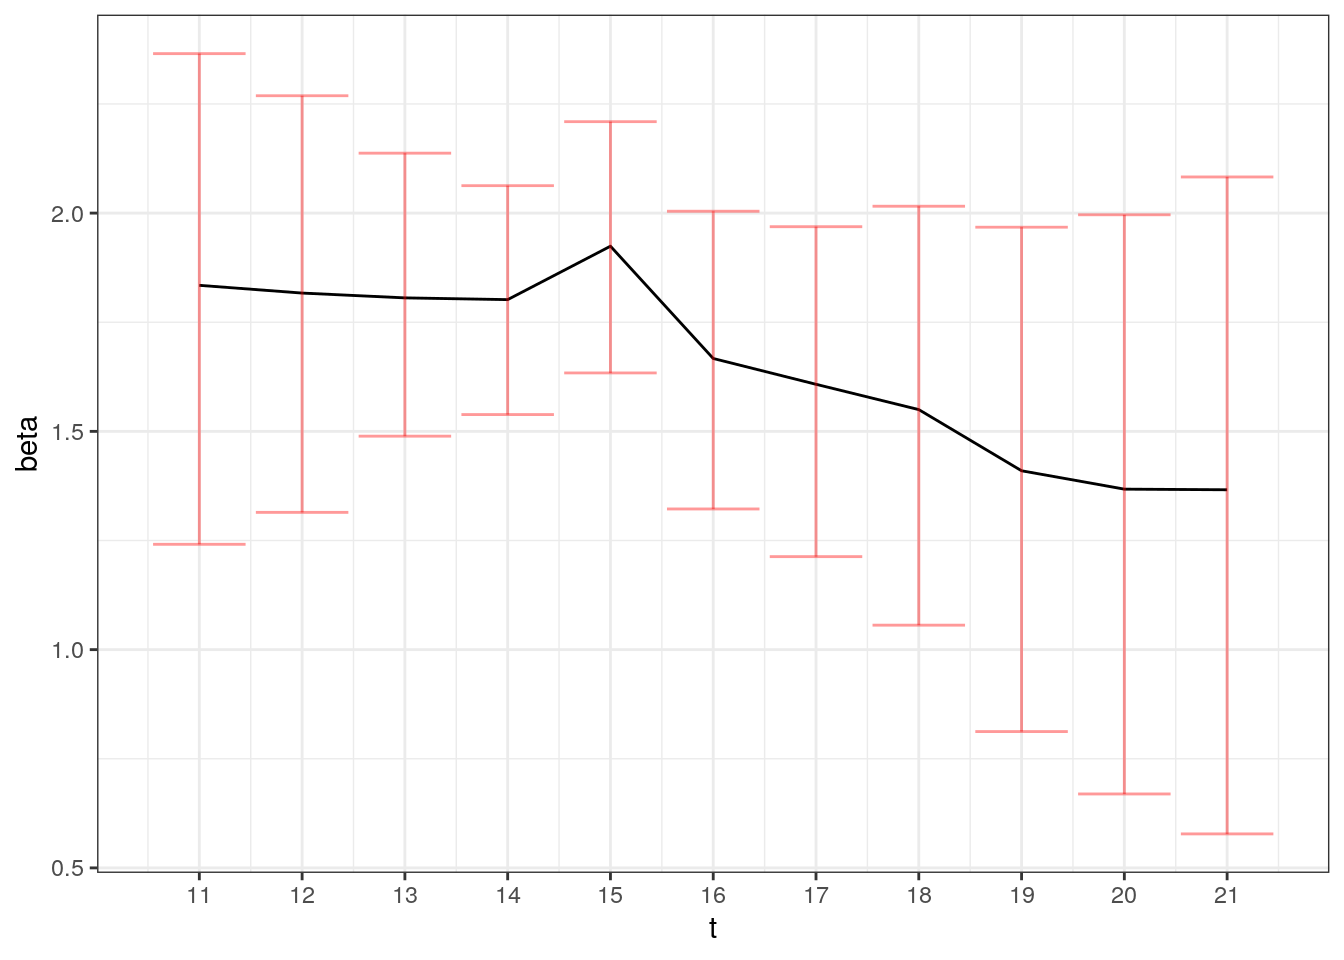
\includegraphics[scale = 0.6]{../figs/corona--plot-coefficients2-1.pdf}
  \end{figure}
\end{frame}

\begin{frame}{Geobserveerde (vaste lijn) en verwachte sterfte (gestipte lijn) 2020, sterfte 2013 - 2019 (grijze lijnen) }
\begin{figure}
\centering
\includegraphics[scale = 0.6]{../figs/corona--oversterfte3-1.pdf}
\end{figure}
\end{frame}

\begin{frame}{Oversterfte per week, 4 modellen}
\begin{figure}
\centering
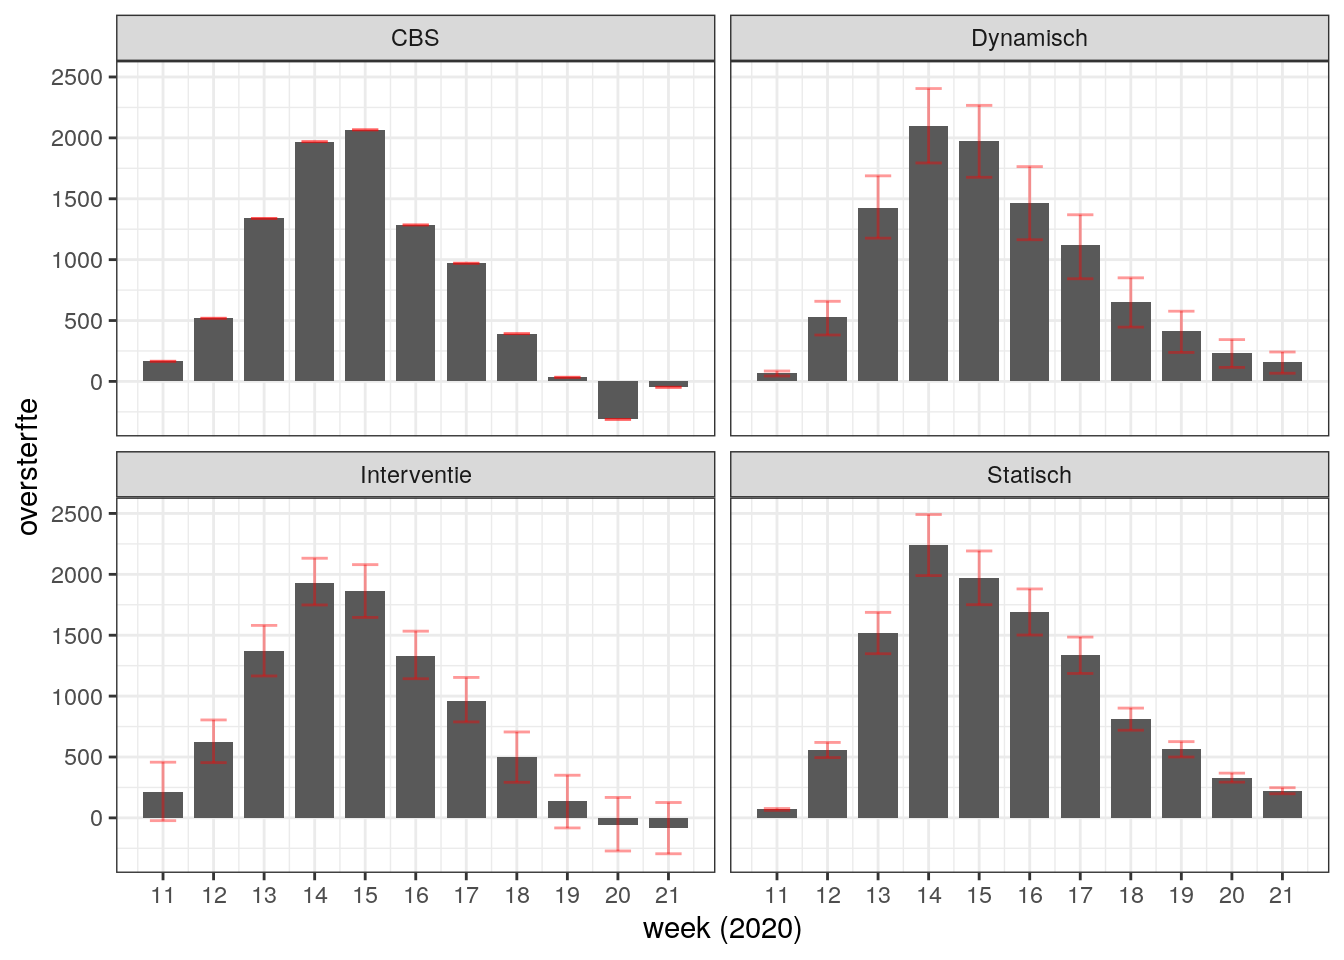
\includegraphics[scale = 0.6]{../figs/corona--oversterfte4-1.pdf}
\end{figure}
\end{frame}

\begin{frame}{Totale oversterfte, week 11 tom week 19}
\begin{figure}
\centering
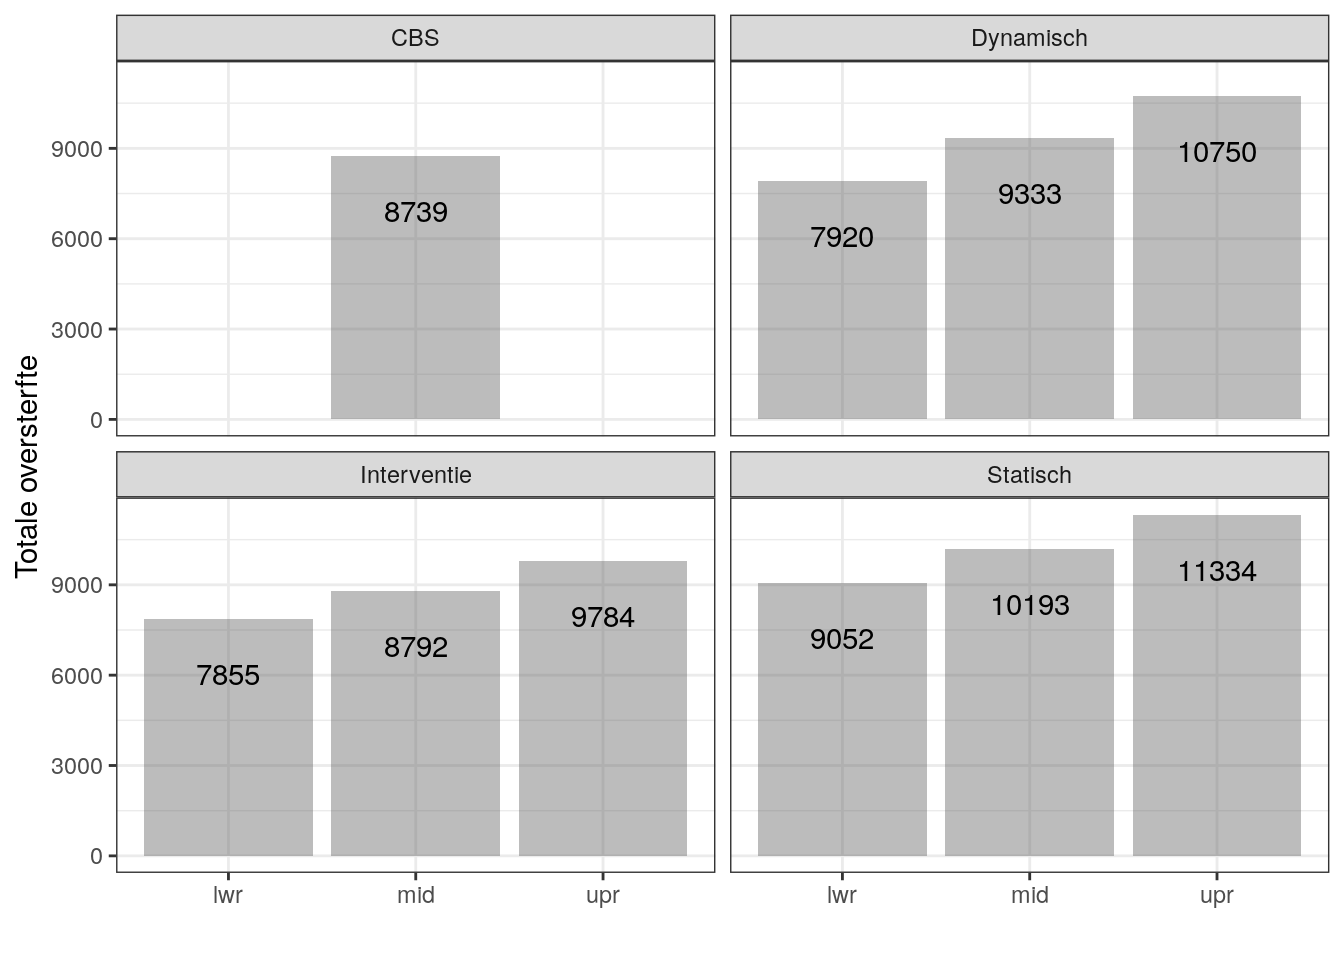
\includegraphics[scale = 0.6]{../figs/corona--oversterfte5-1.pdf}
\end{figure}
\end{frame}

\begin{frame}{Conclusies}
    \begin{itemize}
    \item De totale oversterfte komt aardig in de buurt van de cijfers van het CBS
    \item Volgens onze betrouwbaarheidsinterval ligt het aantal sterfgevallen door het coronavirus tussen de 7000 en de 10500
      \item Het gebruik van een statisch regressiemodel geeft veel hoger inschatting van oversterfte. De dynamische parameters geven flexibiliteit en in deze context lijkt dat noodzakelijk
      \item Volgens onze model is er geen sprake van ondersterfte in weken 20 en 21 maar de coefficienten zijn ook niet significant. Ondersterfte komt dan terecht in het ruis
    \end{itemize}
  \end{frame}

\begin{frame}{Het model}
  \[
\begin{aligned}
&y_{t} = \alpha_{t} + \beta_{t} x_{t} + g_{t} + y_{t}^{ar} + v_{t} & v_{t} \sim N(0, \sigma_{v}^{2}) \\
&\alpha_{t} = \alpha_{t-1} + w_{\alpha, t} & w_{\alpha, t} \sim N(0, \sigma_{\alpha}^{2}) \\
&\beta_{t} = \beta_{t-1} + w_{\beta, t} & w_{\beta, t} \sim N(0, \sigma_{\beta}^{2}) \\
&g_{t} = \sum_{j=1}^{2} \left( a_{j} \cos \left( t \frac{2 \pi j}{52.18} \right) + b_{j} \sin \left( t \frac{2 \pi j}{52.18} \right) \right) + w_{g, t} & w_{g, t} \sim N(0, 0) \\
&y_{t}^{ar} = \phi y_{t-1} + w_{ar,t} & w_{ar,t} \sim N(0, \sigma_{ar}^{2})
\end{aligned}
\]
 \end{frame}

\end{document}
